\section{Dominio de Información}

\insertsectionpage

\begin{frame}[allowframebreaks]

  \frametitle{Dominio de Información}

  \begin{columns}
    \begin{column}{.5\textwidth}
      \begin{itemize}
        \item Los datos puestos en contexto generar información.
        \item La información para lograr un fin genera conocimiento.
        \item El conocimiento aplicado a acciones concretas da lugar a sabiduría.
      \end{itemize}
    \end{column}

    \begin{column}{.5\textwidth}
      \begin{figure}[ht]
        \centering
        \includegraphics[width=1\textwidth]{img/Pirámide.png}
        \caption{\label{fig:dominio-piramide} Pirámide del conocimiento.\cite{MinTIC2021}}
      \end{figure}
    \end{column}
  \end{columns}
  
  \begin{figure}[ht]
    \centering
    \includegraphics[width=\textwidth]{img/Pirámide2.png}
    \caption{\label{fig:dominio-piramide-2} Pirámide del conocimiento, ejemplo trivial\cite{MinTIC2021}}
  \end{figure}

\end{frame}

\section{Lineamientos}

\insertsectionpage

\begin{frame}[allowframebreaks]

  \frametitle{Gobierno de la información}

  \begin{columns}
    \begin{column}{.5\textwidth}
      \begin{itemize}
        \item Las entidades públicas deben establecer un modelo de gobierno que regule políticas, responsabilidades, decisiones y métricas para controlar la información.
      \end{itemize}  
    \end{column}

    \begin{column}{.5\textwidth}
      \begin{figure}[ht]
        \centering
        
\includegraphics[width=0.8\textwidth]{img/GobiernoDatos.jpg}
        \caption{Imagen sacada de Bermejo Eduardo\cite{bermejo2023claves}}
      \end{figure}

    \end{column}
  \end{columns}  


\end{frame}

\begin{frame}[allowframebreaks]

  \frametitle{Gestión de la calidad de los datos}

  \begin{columns}
    \begin{column}{.5\textwidth}
      \begin{itemize}
        \item Las entidades públicas deben crear una estrategia que permita evaluar y mejorar la calidad de la información para apoyar la toma de decisiones.
      \end{itemize}  
    \end{column}

    \begin{column}{.5\textwidth}
      \begin{figure}[ht]
        \centering
        
\includegraphics[width=\textwidth]{img/DataQuality.png}
        \caption{Imagen sacada de \textit{Huawei Enterprise Community}\cite{huawei2023gestion}}
      \end{figure}

    \end{column}
  \end{columns}  


\end{frame}

\begin{frame}[allowframebreaks]

  \frametitle{Gestión de documentos electrónicos}

  \begin{columns}
    \begin{column}{.5\textwidth}
      \begin{itemize}
        \item Las entidades públicas deben implementar un programa para organizar y controlar documentos y expedientes electrónicos de forma eficiente.
      \end{itemize}  
    \end{column}

    \begin{column}{.5\textwidth}
      \begin{figure}[ht]
        \centering
        
\includegraphics[width=\textwidth]{img/GestionDocumentos.jpg}
        \caption{Imagen sacada de \textit{Exact}\cite{Exact2022}}
      \end{figure}

    \end{column}
  \end{columns}  


\end{frame}

\begin{frame}[allowframebreaks]

  \frametitle{Marco de Referencia Geoespacial}

  \begin{columns}
    \begin{column}{.5\textwidth}
      \begin{itemize}
        \item Las entidades públicas deben seguir las directrices del Marco de Referencia Geoespacial de la ICDE para facilitar la gestión geoespacial.
        \item Disponible en \url{https://www.icde.gov.co/marcos/marco-de-referencia-geoespacial}
      \end{itemize}  
    \end{column}

    \begin{column}{.5\textwidth}
      \begin{figure}[ht]
        \centering
        
\includegraphics[width=\textwidth]{img/ICDE.png}
        \caption{Logo de la ICDE\cite{ICDE2025}}
      \end{figure}

    \end{column}
  \end{columns}  


\end{frame}

\begin{frame}[allowframebreaks]

  \frametitle{Publicación de los servicios de intercambio de información}

  \begin{columns}
    \begin{column}{.5\textwidth}
      \begin{itemize}
        \item Las entidades de la administración pública deben exponer sus servicios de intercambio de información a través de la Plataforma de Interoperabilidad del Estado colombiano.
        \item A la fecha la plataforma se encuentra caída \url{https://lenguaje.mintic.gov.co/}.
      \end{itemize}  
    \end{column}

    \begin{column}{.5\textwidth}
      \begin{figure}[ht]
        \centering
        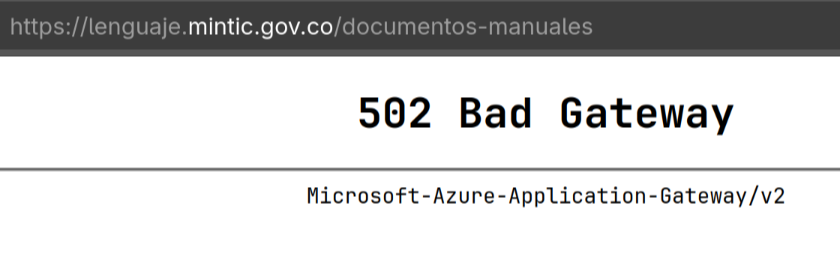
\includegraphics[width=\textwidth]{img/502.png}
        \caption{Plataforma de Interoperabilidad del Estado Colombiano\cite{MinTIC_MarcoInteroperabilidad}}
      \end{figure}

    \end{column}
  \end{columns}  


\end{frame}

\begin{frame}[allowframebreaks]

  \frametitle{Explotación de datos}

  \begin{columns}
    \begin{column}{.5\textwidth}
      \begin{itemize}
        \item Las entidades de la administración pública deben seleccionar técnicas y herramientas que faciliten el análisis de los datos, habilitando la toma de decisiones en base a información de calidad.
        \item Para la manipulación de datos el gobierno recomienda el uso de Software Libre.
      \end{itemize}  
    \end{column}

    \begin{column}{.5\textwidth}
      \begin{figure}[ht]
        \centering
        
\includegraphics[width=\textwidth]{img/SoftwareLibre.png}
        \caption{Imagen sacada del MinTIC\cite{MinTIC_SoftwareLibre}}
      \end{figure}

    \end{column}
  \end{columns}


\end{frame}


\section{Etapas}

\insertsectionpage


\begin{frame}[allowframebreaks]

  \frametitle{Etapas}

  
  \begin{figure}[ht]
    \centering
    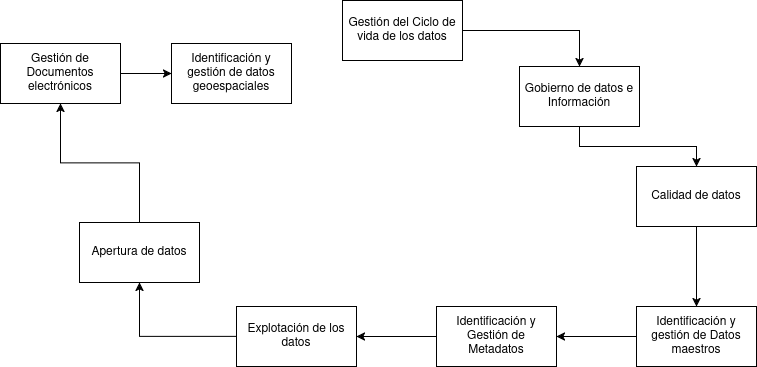
\includegraphics[width=0.6\textwidth]{img/Etapas.png}
    \caption{Información sacada de MGGTI.G.GI\cite{MinTIC2021}. Diagrama realizado por los autores.}
  \end{figure}

  


\end{frame}

\section{Roles}

\insertsectionpage

\begin{frame}[allowframebreaks]

  \frametitle{Roles}

  Roles presentes durante la gestión del ciclo de vida de los datos.\cite{MinTIC2021}

\begin{columns}
  \begin{column}{.5\textwidth}
    \begin{itemize}
      \item Arquitecto Empresarial.
      \item Arquitecto de Información.
      \item Analista de calidad de datos.
      \item Administrador de datos.
    \end{itemize}
  \end{column}

  \begin{column}{.5\textwidth}
    \begin{itemize}
      \item Dueño de datos.
      \item Administrador de bases y respositorios de datos.
      \item Oficial de protección de datos personales.
      \item Analista o científico de datos.
    \end{itemize}
  \end{column}


\end{columns}


\end{frame}




  


